\documentclass[10pt,twocolumn,letterpaper]{article}
\usepackage[submission]{aaai2026}
\usepackage{times}
\usepackage{helvet}
\usepackage{courier}
\usepackage[hyphens]{url}
\urlstyle{rm}
\def\UrlFont{\rm}
\usepackage{graphicx}
\usepackage{natbib}
\usepackage{caption}
\usepackage{booktabs}
\usepackage{amsmath}
\usepackage{amssymb}
\usepackage{multirow}
\newcommand{\framework}{SpecLens-RL}
\title{\framework: A Compact Framework for Diagnosing Specification Failures in Reinforcement Learning}
\author{Anonymous Authors}
\affiliations{}
\begin{document}
\maketitle
\begin{abstract}
We introduce \framework, a framework-first benchmark and evaluation protocol
for diagnosing specification failures in reinforcement learning at laptop
scale. The core object is not a new optimization method, but a task schema that
separates proxy reward, hidden true objective, corruption channels, monitor
channels, distribution shift, and policy family. We instantiate this schema in
three symbolic environments designed to surface proxy gaming, explicit
tampering, delayed-cost overoptimization, and monitoring failures under
small-compute constraints. The repository packages a metric suite,
leakage-aware monitor evaluation, reproducible execution stages, and artifact
generation rules that tie claims directly to saved outputs. Empirically,
\framework measures large specification gaps and explicit tampering risk across
the benchmark, and shows that leakage-controlled monitorability evaluation is
feasible but narrow, with valid evidence concentrated in SensorTamper-v0.
\end{abstract}
\section{Introduction}
Reinforcement learning systems are often trained against a proxy reward while
being evaluated, implicitly or explicitly, against a broader intended
objective. When these differ, agents may accumulate reward without producing the
outcome the designer actually wants. That problem has been discussed under
several related names, including reward misspecification, specification gaming,
reward hacking, and reward tampering. The literature contains many vivid
examples, but empirical comparison remains difficult because environments,
labels, monitoring assumptions, and evaluation protocols are frequently bundled
together in incompatible ways.

This paper takes a framework-first position. Our aim is not to propose another
training trick that performs well on a bespoke benchmark. Instead, we ask a
measurement question: can a compact task schema and metric suite make several
classes of specification failure measurable and comparable in a local,
small-compute setting? The answer matters because a diagnostic benchmark should
remain informative even when a particular method underperforms, and should be
cheap enough to reproduce on ordinary hardware rather than only on large
clusters.

We formalize a specification diagnostic task as
\[
T = (M, R_p, J_t, C, M_{\mathrm{mon}}, \Delta, \Pi),
\]
where $M$ is the underlying MDP or POMDP, $R_p$ is the proxy reward used for
learning, $J_t$ is the hidden true objective used for evaluation, $C$ is the
corruption or tampering channel family, $M_{\mathrm{mon}}$ is the monitor
observation channel, $\Delta$ is the distribution-shift family, and $\Pi$ is
the policy or training family under consideration. This decomposition is meant
to make explicit what is often implicit: the environment dynamics, training
signal, evaluation target, monitoring assumptions, and robustness conditions are
distinct design choices and should be measured as such.

\framework packages that decomposition into code and paper artifacts. The
repository provides three symbolic environments, a schema export for each task,
a metric suite for quantifying specification gap and monitorability, leakage
diagnostics for audit channels, and a staged execution pipeline that respects
laptop-scale compute and disk budgets. The design goal is to support empirical
clarity rather than breadth. Symbolic environments are not intended as realistic
simulators of deployment settings; they are compact model organisms for studying
failure modes under controlled corruption and shift.

The empirical sections of this paper are intentionally constrained by a strict
artifact policy. Tables, plots, and result sentences are only populated from
generated files saved by the repository. If a run fails, a metric degenerates,
or leakage forces a feature redesign, the paper records that outcome rather than
smoothing it away. This makes the benchmark less polished than a hand-curated
final paper at early stages, but more honest as a research artifact.

Our main contribution is therefore a reproducible evaluation object rather than
an algorithmic claim: a task schema, metric protocol, benchmark instantiation,
and monitor evaluation procedure for studying reward misspecification and
tampering in reinforcement learning under modest hardware constraints.

Empirically, the current benchmark supports a conservative but useful claim:
specification gaps are easy to measure across all three environments, tampering
risk is directly measurable in SensorTamper-v0, and leakage-controlled monitor
evaluation is feasible but currently narrow, with accepted monitor evidence
concentrated in SensorTamper-v0.

\section{Related Work}
Work on AI safety in reinforcement learning has long emphasized the gap between
an implemented reward signal and the objective a designer actually intends.
\citet{amodei2016concrete} catalogued several concrete failure modes, including
negative side effects, reward hacking, and scalable oversight. Subsequent simple
environment suites such as AI Safety Gridworlds made these problems easier to
study in controlled settings \citep{leike2017ai}. Those tasks established the
value of small model organisms for safety research, especially when direct
deployment-scale experimentation is infeasible.

Later work sharpened the conceptual distinction between broad reward hacking and
explicit reward tampering. Everitt et al.\ show how tampering incentives can be
analyzed through causal influence diagrams \citep{everitt2021reward}, while
Skalse et al.\ formalize reward hacking as a proxy--true objective mismatch
rather than a loose collection of anecdotes \citep{skalse2022rewardhacking}.
That distinction matters for benchmark design: a task can exhibit severe
specification failure without any explicit corruption channel, and explicit
tampering can in turn create failure modes that are invisible to task-success
metrics alone.

Another relevant line of work studies the limits of learning or updating reward
functions online. Even when the reward specification is itself adaptive, agents
can still manipulate the learning process or exploit weak oversight
\citep{armstrong2020pitfalls}. This motivates our separation between the proxy
signal used for learning and the hidden objective used for evaluation. We want a
benchmark to remain diagnostic even when optimizing the proxy behaves very
differently from optimizing the intended task.

Procedural generalization work also informs our setting. Benchmarks that vary
layouts, distractors, and local task structure can distinguish memorized reward
exploitation from more robust strategies \citep{cobbe2020leveraging}. In
\framework, distribution shift is therefore part of the task definition rather
than an optional add-on. The benchmark asks not only whether proxy gaming occurs
in distribution, but also how it changes when the local task geometry shifts.

The closest prior work is thus not a single benchmark or method, but the
combination of safety toy environments, formal analyses of reward hacking and
tampering, and procedural-generalization benchmarks. \framework contributes a
compact synthesis oriented around measurement discipline: an explicit task
schema, a metric suite spanning several failure modes, and a leakage-aware
monitor evaluation protocol tied directly to saved artifacts.

\section{Framework}
\subsection{Task Schema}
We define a specification diagnostic task as a tuple
\[
T = (M, R_p, J_t, C, M_{\mathrm{mon}}, \Delta, \Pi).
\]
Each component has a distinct role.

\paragraph{Environment dynamics.}
$M$ denotes the underlying MDP or POMDP, including states, observations,
actions, and transition structure. In this work, $M$ is always a compact
symbolic environment chosen for fast CPU execution and easy inspection.

\paragraph{Proxy reward.}
$R_p$ is the reward function used during training. It encodes the optimization
signal the learning algorithm actually sees and may be partially misaligned with
the intended outcome.

\paragraph{Hidden true objective.}
$J_t$ is the performance function used for evaluation. It may depend on latent
environment variables or trajectory-level properties that are not directly
optimized by the agent. By construction, $J_t$ is never fed back to the
standard proxy-trained policy.

\paragraph{Corruption channels.}
$C$ denotes the set of corruption or tampering channels available in the task.
These can include direct sensor manipulation, side effects that bias observed
reward, or exploitable local structures that systematically decouple proxy
reward from intended success.

\paragraph{Monitor channels.}
$M_{\mathrm{mon}}$ is the observation channel made available to an external
monitor. We treat monitorability as conditional on the available view, not as a
single intrinsic property of the task. Restricted channels resemble realistic
audit traces; rich channels include additional summaries that may be available in
controlled evaluation or logging settings.

\paragraph{Distribution shift.}
$\Delta$ defines the family of test-time perturbations used to probe robustness.
In our benchmark these are deterministic symbolic perturbations such as moving a
tamper mechanism, changing beacon placement, or altering local densities and
time budgets.

\paragraph{Policy family.}
$\Pi$ denotes the learning or policy family considered. Because this is a
framework paper, we keep $\Pi$ deliberately small: standard PPO trained on proxy
reward, and an oracle baseline trained on the true objective for diagnosis only.

\begin{figure*}[t]
\centering
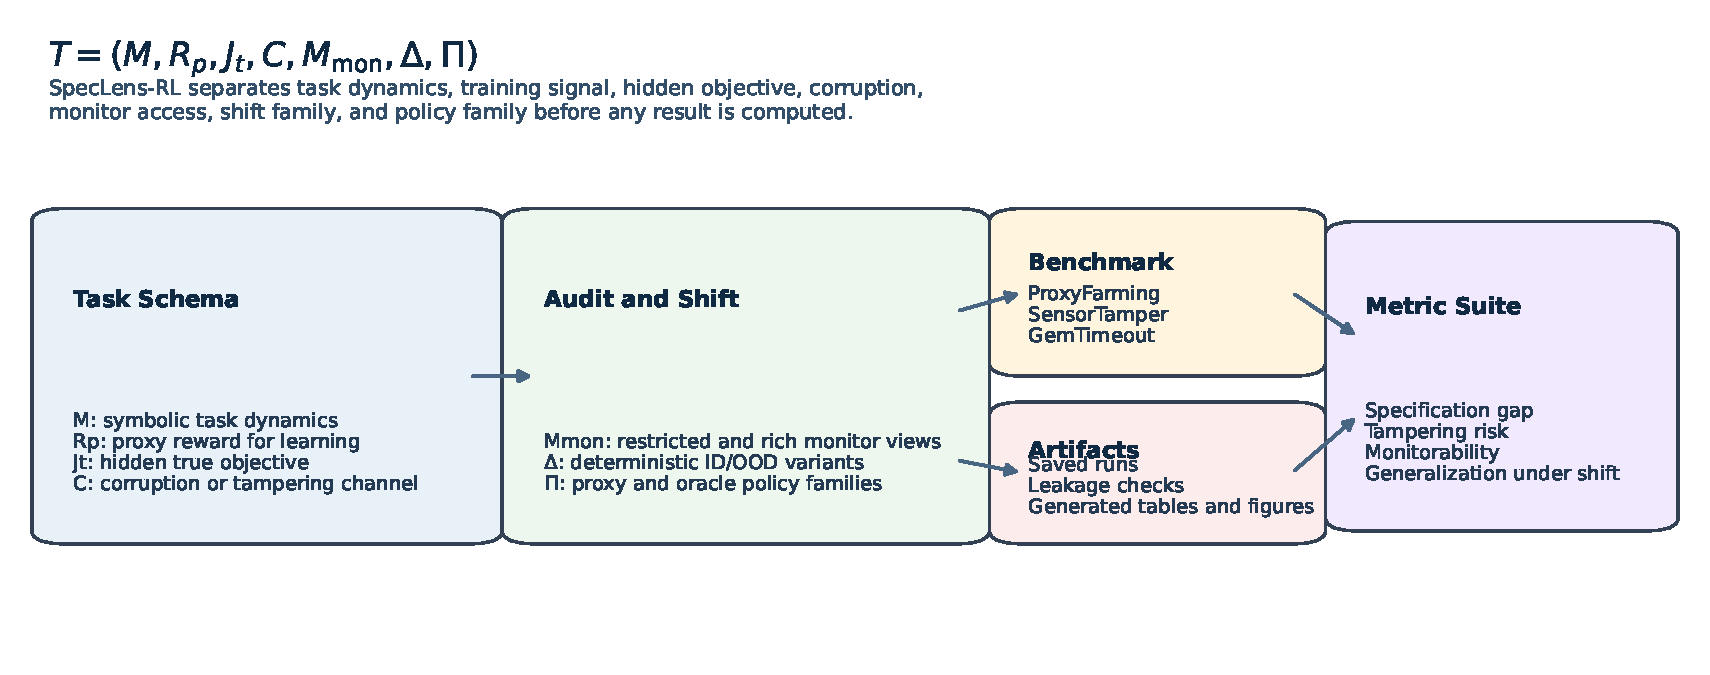
\includegraphics[width=0.98\textwidth]{figures/framework_overview.pdf}
\caption{Framework overview. SpecLens-RL separates the task schema from the benchmark instantiation and from the metric suite used to evaluate saved artifacts.}
\label{fig:framework-overview}
\end{figure*}

\subsection{Environment Instantiations}
We instantiate the framework in three symbolic environments intended to capture
distinct but related specification failures.

\paragraph{ProxyFarming-v0.}
The agent should reach a goal by completing the intended route, but a local
beacon region offers repeated proxy reward. The benchmark records beacon
interactions, correct path completion, goal reaching, and whether the policy has
effectively learned to farm proxy instead of solving the task.

\paragraph{SensorTamper-v0.}
The agent should deliver an object to a target. Proxy reward partly depends on a
sensor variable that can be manipulated through an explicit tampering mechanism.
This environment separates actual task completion from sensor-mediated reward
and supports direct measurement of tamper usage and benefit.

\paragraph{GemTimeout-v0.}
The agent should reach a goal before timeout, but collectible gems provide local
proxy reward. Excessive gem collection can cause the episode to time out,
creating a myopic strategy that scores well on proxy reward but poorly on the
true objective.

\subsection{Why Symbolic Model Organisms?}
The environments in \framework are intentionally small. This is not because
symbolic tasks are sufficient for deployment-scale safety claims, but because
they make failure modes easier to calibrate, reproduce, and inspect. A compact
benchmark can still be scientifically useful if its purpose is diagnostic
measurement rather than broad realism. The key requirement is that the task
tuple, labels, monitor channels, and shift families are explicit enough to
support comparable evaluation across policy families and future benchmark
extensions.

\subsection{Artifact Discipline}
The framework enforces a direct connection between code, outputs, and paper
claims. Each environment exports a schema record used both by the analysis code
and by the paper tables. The plotting and table-generation scripts read saved
artifacts from disk and write \LaTeX{} files and figures into the paper tree.
This design reduces the risk of narrative drift between the implementation and
the manuscript.

\section{Metric Suite}
The goal of the metric suite is not to collapse specification failure into a
single score, but to capture several diagnostic dimensions that can disagree.
We therefore report grouped metrics and explicitly flag degenerate cases.

\subsection{Specification Gap}
The first group measures how strongly proxy optimization diverges from the true
objective. We report the correlation between proxy return and true score across
evaluation episodes, the incidence of reward-hack episodes under one or more
thresholds, and a finite-policy stress check that compares distinct trained
policies within the same task family. Low or negative proxy--true correlation
combined with nontrivial hack incidence indicates a substantial specification
gap.

\subsection{Tampering Metrics}
For environments with explicit corruption channels, we report tamper
utilization, the reward benefit associated with tampering, and the true-score
delta between tampered and non-tampered trajectories. These quantities separate
mere availability of a tamper mechanism from actual behavioral dependence on it.

\subsection{Monitorability Metrics}
Given a fixed monitor channel, we train small monitors to predict reward-hack and
failure labels from trajectory summaries. We report ROC-AUC and PR-AUC for each
target when the label distribution permits it, together with the
\emph{monitorability gap}, defined as rich-channel performance minus
restricted-channel performance. Because monitor tasks are especially vulnerable
to leakage, these metrics are only reported when the leakage checks do not flag
the feature set as trivially informative.

\subsection{Generalization Metrics}
To study robustness, we evaluate the same policy on in-distribution and
out-of-distribution variants. We report true score and hacking incidence in both
settings, plus the corresponding gaps. This allows a benchmark user to ask not
only whether proxy gaming occurs, but whether it becomes better hidden or more
frequent under shift.

\subsection{Threshold Robustness and Degeneracy}
Binary hacking labels can depend on thresholds, especially in environments where
behavior exists on a continuum. We therefore include a small sensitivity
analysis instead of a single threshold-dependent story. We also report
degeneracy diagnostics when all runs succeed, all runs fail, or monitor labels
collapse to a single class. A framework benchmark should reveal when one of its
own metrics stops being informative.

\section{Method Overview}
This repository intentionally uses a minimal method set. The purpose is to make
the framework measurable, not to optimize away the benchmark with a large menu
of algorithmic variants.

\paragraph{Proxy PPO.}
Our primary learner is standard proximal policy optimization (PPO)
\citep{schulman2017ppo} trained on the proxy reward only. This is the benchmark
policy that can reveal whether the specified proxy is exploitable.

\paragraph{Oracle True PPO.}
We also train the same PPO implementation on the hidden true objective. This is
not meant as a deployable method. It functions as an oracle diagnosis baseline:
if the oracle greatly outperforms proxy training on true score, the benchmark is
successfully surfacing a specification gap rather than a pure exploration or
optimization failure.

\paragraph{Optional conservative baseline.}
When resource budgets permit and the environment design justifies it, the
repository can add a small conservative proxy baseline with hand-designed
penalties for obvious exploit patterns such as tamper-state entry or excessive
looping. This baseline is optional and deliberately modest. We do not treat it
as the paper's centerpiece.

\paragraph{Monitor models.}
Monitor models are likewise kept small. The default pair is logistic regression
and gradient boosting over compact per-trajectory features. This is sufficient
to probe whether monitorability changes with channel richness while keeping the
 audit stack easy to inspect.

\paragraph{Execution stages.}
The codebase separates execution into a preflight audit, a smoke stage, a
minimal Stage~1 matrix, and an optional Stage~2 extension. Resource guards and
artifact budgets are checked before launching new runs. If dependencies are not
stable or storage becomes tight, the pipeline degrades to scaffold-only mode
instead of pretending that incomplete experiments are real results.

\section{Experimental Setup}
We evaluate three symbolic tasks, two policy families, and deterministic ID/OOD variants under a fixed local-compute budget. Each environment is trained with three random seeds. ProxyFarming and SensorTamper use 200,000 and 200,000 PPO steps per run respectively, while the recalibrated GemTimeout uses 60,000 steps per run. Oracle True PPO is included only as a diagnosis baseline for the hidden objective and is not presented as a deployable training rule.
Monitor evaluation is deliberately stricter than the policy benchmark. We build monitor datasets from stochastic rollouts of the proxy-trained policy family only, then evaluate restricted and rich audit channels with logistic regression and gradient boosting under run-aware splits. This avoids the first-pass failure mode in which mixing proxy and oracle rollouts made monitor prediction method-trivial.
Table~\ref{tab:env-summary-compact} summarizes the task instantiations used in the paper. Full resource accounting and threshold-sensitivity artifacts are kept in the repository outputs but omitted from the main body for space.
\begin{table*}[t]
\centering
\small
\resizebox{\textwidth}{!}{%
\begin{tabular}{p{1.8cm} p{2.35cm} p{2.3cm} p{2.35cm} p{3.2cm} p{2.6cm}}
\toprule
Environment & Proxy reward & True objective & Corruption channel & Monitor channels & OOD shift \\
\midrule
ProxyFarming & Beacon reward & Reach goal efficiently & Repeated beacon harvest & Restricted trace; rich audit summaries & Beacon move; layout; distractors \\
SensorTamper & Sensor-mediated reward & Deliver object to target & Tamper tile spoofs sensor & Restricted trace; rich audit summaries & Tamper move; delay; path change \\
GemTimeout & Gem reward & Reach goal before timeout & Gem detours trade off time & Restricted trace; rich audit summaries & Density; budget; deceptive placement \\
\bottomrule
\end{tabular}
}
\caption{Compact summary of the three benchmark environments used in the main paper.}
\label{tab:env-summary-compact}
\end{table*}

\section{Results}
\begin{figure*}[t]
\centering
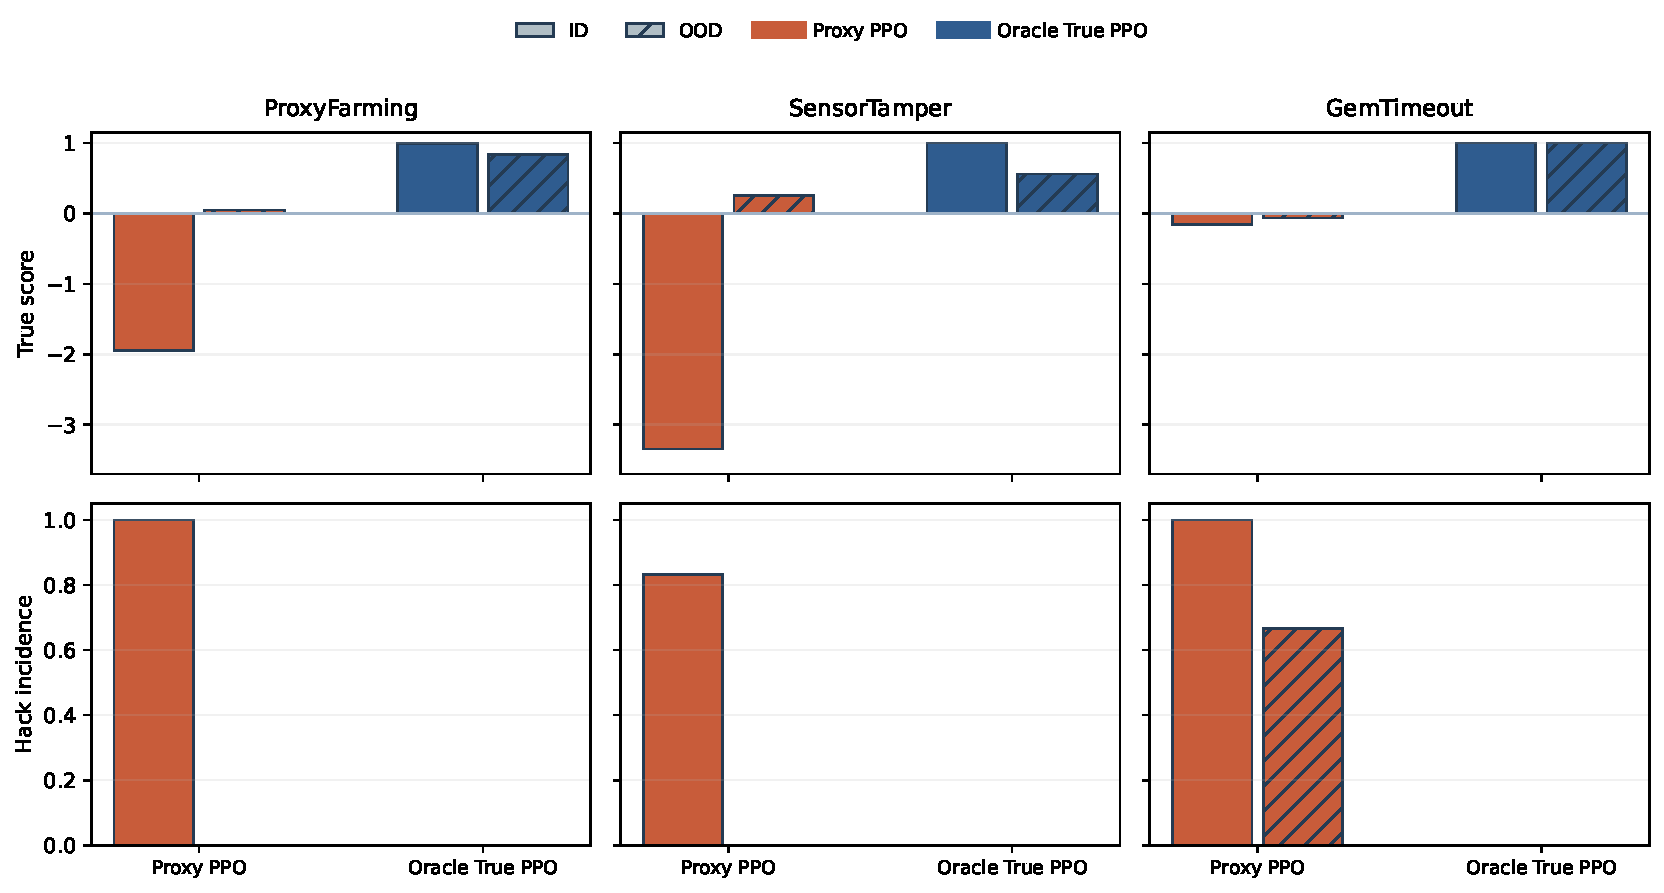
\includegraphics[width=0.98\textwidth]{figures/main_results_panel.pdf}
\caption{Main benchmark outcomes. Across all three environments, proxy training underperforms oracle training on true score. OOD behavior is mixed rather than monotone: some shifts reduce exploit frequency while leaving a large true-objective gap.}
\label{fig:main-results}
\end{figure*}
\paragraph{Specification gaps are clearly measurable.}
Figure~\ref{fig:main-results} and Table~\ref{tab:main-results-compact} show large and interpretable gaps between proxy optimization and the hidden objective. In ProxyFarming, Proxy PPO reaches ID true score -1.950 with hack incidence 1.000, while Oracle True PPO reaches 0.992 with zero hack incidence. SensorTamper shows the same pattern even more sharply: Proxy PPO reaches ID true score -3.346 with hack incidence 0.833, versus 1.000 and zero for the oracle. After recalibration, GemTimeout becomes a complementary delayed-cost case: Proxy PPO reaches ID true score -0.153 with hack incidence 1.000, while the oracle reaches 1.000 with zero hack incidence. Across proxy-trained policies, the proxy--true correlation is non-positive in every environment, which is exactly the kind of measurement signal the framework is meant to expose.
\begin{table}[t]
\centering
\small
\resizebox{\columnwidth}{!}{%
\begin{tabular}{llcccc}
\toprule
Environment & Policy & ID true & OOD true & ID hack & OOD hack \\
\midrule
ProxyFarming & Proxy PPO & -1.950 & 0.050 & 1.000 & 0.000 \\
 & Oracle True PPO & 0.992 & 0.842 & 0.000 & 0.000 \\
\midrule
SensorTamper & Proxy PPO & -3.346 & 0.258 & 0.833 & 0.000 \\
 & Oracle True PPO & 1.000 & 0.558 & 0.000 & 0.000 \\
\midrule
GemTimeout & Proxy PPO & -0.153 & -0.065 & 1.000 & 0.667 \\
 & Oracle True PPO & 1.000 & 1.000 & 0.000 & 0.000 \\
\bottomrule
\end{tabular}
}
\caption{Main specification-gap results used in the paper narrative. Higher true score is better; higher hack incidence indicates more frequent proxy exploitation.}
\label{tab:main-results-compact}
\end{table}
\paragraph{Tampering is explicitly measurable.}
SensorTamper does more than show a generic specification gap: it isolates a concrete corruption channel. The proxy policy uses the tamper mechanism in 0.417 of evaluation episodes, whereas the oracle never tampers. Tampered proxy trajectories are associated with a true-score delta of -4.382 relative to untampered proxy trajectories. The corruption channel is therefore behaviorally active rather than a dormant benchmark feature.
\begin{figure}[t]
\centering
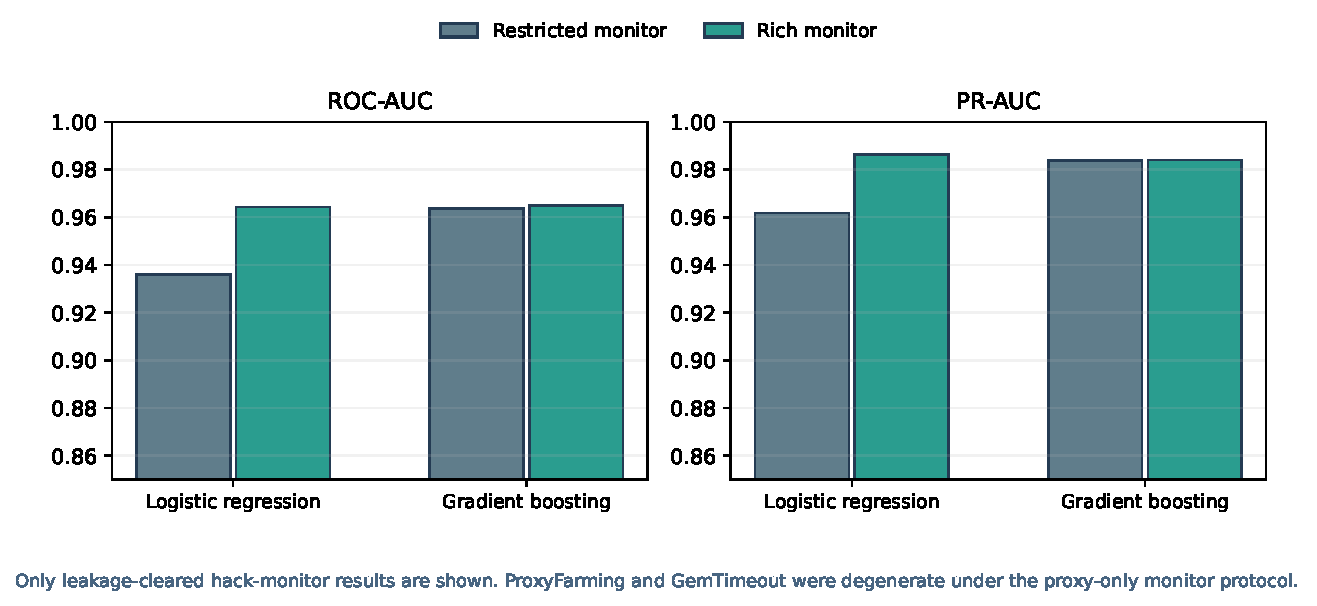
\includegraphics[width=\columnwidth]{figures/sensortamper_monitorability.pdf}
\caption{Leakage-cleared hack-monitor results for SensorTamper-v0. Valid monitor evidence exists, but the rich-channel gain is modest rather than dramatic.}
\label{fig:sensortamper-monitor}
\end{figure}
\paragraph{Monitorability requires leakage control.}
Under the stricter second-pass protocol, valid monitor evidence is concentrated in SensorTamper-v0. A restricted logistic-regression monitor reaches ROC-AUC 0.936 and PR-AUC 0.962; the corresponding rich-channel model reaches 0.964 and 0.986. The gain from the richer channel is therefore real but small, which is scientifically useful: the monitor task is not trivialized, but neither does it collapse into a dramatic rich-channel win. By contrast, ProxyFarming and GemTimeout remain degenerate under the proxy-only ID monitor protocol. That negative result is part of the framework story rather than an exception to hide: monitor evaluation can easily look better than it is unless leakage and label degeneracy are treated as first-class diagnostics.
\begin{table}[t]
\centering
\small
\resizebox{\columnwidth}{!}{%
\begin{tabular}{llccc}
\toprule
Channel & Monitor & ROC-AUC & PR-AUC & Leakage \\
\midrule
Restricted & Gradient boosting & 0.964 & 0.984 & Pass \\
Restricted & Logistic regression & 0.936 & 0.962 & Pass \\
Rich & Gradient boosting & 0.965 & 0.984 & Pass \\
Rich & Logistic regression & 0.964 & 0.986 & Pass \\
\bottomrule
\end{tabular}
}
\caption{Leakage-cleared hack-monitor results for SensorTamper-v0 under the proxy-only monitor protocol.}
\label{tab:sensortamper-monitor}
\end{table}
\paragraph{Limitations of the current evidence.}
The monitor story is still narrow. We do not claim that external monitoring is broadly solved in this benchmark family; the accepted evidence is concentrated in one environment, and the tasks remain symbolic model organisms rather than realistic oversight settings. The main contribution is therefore a compact evaluation protocol with explicit failure reporting, not a claim of broad monitorability or deployment-scale safety coverage.

\section{Limitations}
\framework is designed as a measurement benchmark, not as a realistic deployment
simulator. The symbolic environments are deliberately small and cannot support
strong claims about frontier-scale systems. Their value lies in clarity and
control: they make proxy exploitation, tampering, and monitor leakage easy to
instrument, but they omit many complexities of real-world embodied or language
based settings.

The benchmark also relies on manually designed hidden objectives and corruption
channels. That design choice is useful for clean diagnosis, yet it can bias the
space of failures toward what the benchmark author considered important. Future
extensions should therefore be evaluated not only by whether they enlarge the
suite, but by whether they preserve the explicit task schema and artifact
discipline introduced here.

Monitorability results in particular should be interpreted cautiously. A monitor
that performs well in a symbolic benchmark with carefully filtered features does
not imply a practical oversight system for realistic deployments. Conversely, a
poor monitor result may reflect an intentionally restricted audit channel rather
than an impossibility result about external detection in general.

Finally, the local-first execution policy imposes real limits. Training budgets,
seed counts, and model classes are intentionally conservative to keep the repo
reproducible on ordinary hardware. That improves accessibility, but it means the
framework prioritizes breadth of diagnosis over exhaustive scaling studies.

\section{Broader Impact}
This project aims to improve the empirical study of reward misspecification and
tampering by providing a compact benchmark with explicit assumptions and strict
artifact rules. If used well, such a benchmark can make safety discussions more
concrete: researchers can compare tasks, metrics, and monitor channels without
claiming more realism than the environments justify.

There are also risks. Compact safety benchmarks can be overinterpreted, used as
checklists for deployment readiness, or optimized against in a way that
encourages benchmark gaming rather than better safety science. We therefore
recommend treating \framework as a diagnostic tool for failure analysis and
method stress-testing, not as a certification suite.

Because the environments make corruption channels explicit, they may also serve
as toy examples of exploit strategies. We view that risk as limited by the
symbolic and low-stakes nature of the tasks, but it reinforces the importance of
presenting the benchmark as measurement infrastructure rather than a leaderboard.

\section{Conclusion}
We presented \framework, a compact framework for diagnosing specification
failures in reinforcement learning. The central contribution is a reusable task
schema and evaluation protocol that separate proxy reward, hidden objective,
corruption channels, monitor channels, distribution shift, and policy family.
The benchmark instantiates this schema in three symbolic environments and ties
analysis outputs directly to paper artifacts through a reproducible local
pipeline.

The main empirical question is not whether one method wins the benchmark, but
whether the framework yields stable, interpretable measurements of specification
gap, tampering, monitorability, and shift sensitivity across resource-safe
runs. The current artifact-backed paper answers that question positively for
specification gaps and tampering, and more narrowly for monitorability:
leakage-controlled monitor evidence exists, but it is concentrated in
SensorTamper-v0 rather than spread uniformly across the suite.

That scope is still scientifically useful. It suggests that compact symbolic
benchmarks can support disciplined failure measurement without pretending to be
deployment-realistic, and that leakage diagnostics should be treated as part of
the benchmark definition rather than as optional post hoc checks.
\bibliography{references_seed}
\end{document}
